\newpage

\begin{figure}[h]
\centering
{\includegraphics[scale=.25]{0345.eps}}
\end{figure}

{\dn
\begin{center}
{\large\bfseries{\dn bhaaratiiyam adhi"saasanam}}\\[10pt]
{\Large\bfseries{\dn saMsk.rtAyogaH}}\\[30pt]
{\Huge\bfseries{\dn pra"snaavalii}}
\end{center}
}

\vskip 3cm

{\rm 
\begin{center}
{\large\bfseries{SANSKRIT COMMISSION}}\\[30pt]
{\large\bfseries{QUESTIONNAIRE}}
\end{center}
}

\vfill

{\dn
\begin{center}
{\dn\Large\bfseries{\dn saMsk.rtaayoga-sacivaalayaH}}\\
{\dn\Large\bfseries{\dn pUnaa {\dn\dnnum 4}}}\\
{\dn\large\bfseries{\dn kaarttika-paur.namaasii, saMvat {\dn\dnnum 2013}, "sakaabdaaH {\dn\dnnum 1878}}}
\end{center}
}

\newpage


{\dn || .o|| viditaM khalu bhavatAM yat bhaaratagatasya saMsk.rtAdhyayanasya sAmpratikIM samavasthAM sarvatodi"saM pari"siilayituM \dn\dnnum 1956 kristAbdasya aktobara-mAse bhAratIyena adhi"sAsanena `saMsk.rtAyogaH'}

{\dn e.saH AyogaH sviiyavividhakArye.su vi"svavidyAlayagataM taditara\-saMsthAgataM ca saMsk.rta"sik.sAvi.sayakaM sAmpratikam AnukUlyaM vilokayi.syati,\break upakalpayi.syati ca tAMstAn upAyavi"se.sAn saMsk.rtAdhyayanasya saMsk.rta-\-saM"sodhanasya ca abhiv.rddhaye |}

\vskip .1cm

{\dn paramparAgatAM saMsk.rta"sik.sApra.nAlIM parIk.sya tatratyAH ke ke vi"se.sAH navIna"sik.sA\-pra.nAlyAm antarbhAvyamAnAH upayujyeran, ityetadapi asO vicArayi.syati |}

\vskip .1cm

{\dn tam enaM vi.sayam adhik.rtya tadvidAM matam AvAhayitum upanyastA iyaM prak.rtena Ayogena pra"snAvalii | iyaM ca pra"snAvalii vipulavi.sayAvagAhinI | tena hi, ye mahAbhAgAH uttarapre.sa.nena anujigh.rk.seyuH, na taiH ava"syameva pratipra"snam uttaram udaahaaryam | yatra vi.sayavi"se.se ye.sAm abhinive"saH saMbandhavi"se.saH vA vi"si.s.taM j~nAnaM vA syAt, tatra te svamataM tadupodbalakaM ca yuktijAtaM samAsena pradar"sayeyuH, iti sarve vyavahartAraH  amyarthyante | diiyamAnam uttaraM j~nApakaM vA yaM pra"snaM sp.r"sati, tasya pra"snasya a"nka.h spa.s.taM nirde"syaH | }

\vskip .1cm

{\dn A"nglabhA.sayA saMsk.rtabhA.sayA vA uttarA.ni dAtavyAni | uttarA.ni ca `sadasya-sacivaH, saMsk.rtAyogaH, pUnA \dn\dnnum 4' etam uddi"sya tathA pre.sa.nIyAni, yathA 12 .disambara, 1956 etat dinaM yAvat prApyeran\,|}

\vskip .1cm

{\dn  idaM ca aparaM vyavahartAraH prArthyante, yat te sve.sAm uttarA.nAm avasAne nijaM samagraM nAma, adhikAram, AvAsasthAnaM ca likheyu.h||}

\medskip

{\rm 
You are aware that the Government of India have appointed (in October 1956) a Sanskrit Commission to consider the question of the present state of Sanskrit Education in India.

\vskip .1cm

The commission will, among other things survey the existing facilities for Sanskrit Education in Universities and non-University institutions and make proposals for promoting the study of Sanskrit, including research, It will also examine the traditional system of Sanskrit Education in order to find out what features from it an be usefully incorporated into the modern system.


With a view to eliciting informed public opinion on the subject, the Commission has issued the present Questionnaire. The Questionnaire convers a wide field of inquiry, and it is not intended that all those who are pleased to send replies should necessarily answer every question. Correspondoents are requested to favour the Commission with their views and suggestions on matters in which they are particulary interested or concerrxed, or of, which they have special knowledge. Reasons, in brief, may please be given in support of the views expressed. The number of the question to which the answer or memorandum relates should be clearly indicated.

Replies, in English or Sanskrit, may be kindly sent to `The Member Secretary, Sanskrit Commission, Poona 4', so as to reach him not later than the 12th of December, 1956. 

Correspindents are requested to give their full names, designations, and addresses at the end of their replies.
}

\newpage

{\dn || a|| sAmAnyaprakara.nam - mUlabhUtAH kecana pra"snAH ||}

\begin{itemize}
  \item[{\dn\dnnum 1}.] {\dn kA bhUmikA kAryavi"se.saH vA saMsk.rtavidA adyatane bhAratasya rA.s.triyajiivane nirvartayitavyaH ?}  
  
  \item[{\dn\dnnum 2}.] \begin{itemize} 
                        \item[({\dn ka})] {\dn saMsk.rtAdhyayanaM prati bhavadiiye kId.r"sii janAnAM sAdhAra.nii manov.rttiH ?}
                        
                        \item[({\dn kha})] {\dn pA.tha"sAlAsu, mahAvidyAlaye.su, vi"svavidyAlaye.su ca pravartamAnAt saMsk.rtAdhyayanAt vyatireke.na, kaiH kaiH upAyAntaraiH bhavadiiye prade"se saMsk.rtavidyAyAH abhiv.rddhiH kriyate, saMsk.rtasAhitye tadanuprA.nitAyAM saMsk.rtau ca AdaraH paripAlyate ?, iid.r"sasya Adarasya abhiv.rddhe"sca arthe ke upAyAH bhavadbhiH sUcyante ?}
                       \end{itemize}
                       
 \item[{\dn\dnnum 3}.] \begin{itemize}
                      \item[({\dn ka})] {\dn mAnavikI sAMsk.rtikI ca saMsk.rtasya anarghatAm Alocya, saMsk.rtAdhyayana\- vi.saye mahiiyaH uddhodhanam AdaraM ca bhAratiiya ga.natantrAnupAlite.su nAgarike.su samutpAdayituM kAn upAyAn upAdeyatvena bhavantaH sUcayeyuH?}
                      
                      \item[({\dn kha})] {\dn kiid.rgbhiH vidhAbhiH `sAhitya - akAdemI' (akhila-\break\-bhAratiiya-sAhitya-pari.sat) janAnAM saMsk.rtavA"nmayA-\break\-dhyayanasya prarocanAya, tadvi.saye ca AdarasaMvardhanAya, sAhAyyaM kartu.m "saknuyAt ? te.su te.su vidyAsthAne.su  pratinidhibhUtAnAM saMsk.rtagranthAnAm (\dn\dnnum 1) A"nglabhA.sAyAM (\dn\dnnum 2) prAde"sikabhA.sAsu ca anuvAdaiH sahak.rtAni svalpa\-mUlyAni  saMskara.nAni kendrAdhi-\-"sAsanasya rAjyAdhi"sAsa\-nAnAM ca dvAre.na  `sAhitya-akAdemii' svayaM prakA"sayet anyaiH vA prakA"syamAnAni puraskuryAt, ityetadvi.saye bhavatAM kiM matam? [yavana-romaka-bhA.sayoH likhitAnAM granthAnAm aa"nglabhA.sAnuvAda-sahak.rta-saMskara-\-.nAnAM pra.na\-yane, `loeba-klAsikala-lAyabrarii' saMsthayA yA\break sarA.niiH anusriyate, sA atra udAhAryA |]}
                      
                      \item[({\dn ga})] {\dn dvitIyasyAM pA~ncavar.sikyAM yojanAyAM saMsk.rta"sik.sAyAH abhivardhanAya ke upAyAH bhavanmate avalambaniiyAH |}
                      \end{itemize} 
\end{itemize}

{\rm 
\section*{{\rm\bfseries A. General-Some Basic Questions}}

\noindent
\begin{itemize}
  
  \item[1.] What special role has Sanskrit to play in the national life of India to-day?
  
  \item[2.] \begin{itemize}
            \item[(a)] How would you characterize the general sentiment in your part of the conuntry towards the study of Sankrit?  
              
              \item[(b)] Apart from its study in P$\bar{a}$tha$\acute{s}\bar{a}$l$\bar{a}$s, Colleges and Universities, in what other ways are the cultivation of Sanskrit and interest in its literature and culture maintained in your part of the country? What steps would you suggest to promote such interest and cultivation?
             \end{itemize}
  \item[3.]\begin{itemize}
           \item[(a)] In view of the humanistic and cultural value of Sanskrit what steps would you sugeest for engendering among the citizens of the Republic of India a greater awareness for and interest in the study of Sanskrit?
           
           \item[(b)] In what ways can the {\textit {Sahitya Akademi}} help to popularize and promote interest in the study of Sanskrit literature? Should the {\textit {Sahitya Akademi}} in your opinion, undertake and encourage the publication by the Center as well as the States, in cheap editions, of representative Sanskrit texts in the different branches of learning, with accompanying translations in (i) English and (ii) the regional languages (in a style like that of the {\textit {Loeb Classical Library}} of Greek and Latin texts in English, for example)?
           
           \item[(c)] What provisions, in your opinion, need be made in the Second Five Year Plan for the promotion of Sanskrit Education?
           \end{itemize}
\end{itemize}           
}

\begin{itemize}
\item[{\dn\dnnum 4}.] \begin{itemize}
                      \item[({\dn ka})] {\dn apyetat bhavatAm abhimataM yat kasmAccidapi  bhAratiiyaat "sik.sApI.thAt samAvartamAnena yuvajanena saMsk.rtasaMsk.rteH biijabhUtaiH a"ngaiH ava"syam Atta\- paricayena bhavitavyam iti?}
                
                     \item[({\dn kha})] {\dn ke ke upAyAH bhavatAM saMmatAH yaiH Ad.rtaiH vide"sagAminaH bahavaH chAtrA: adhikAri.naH, bhAratarA.s.triyakAryAlaye.su niyuktAHkarmacAri.na"sca, nyUnAdhikayA mAtrayA etasyAH saMsk.rteH yathArthatvena paricAyakAH bhaveyuH?}
                
                     \item[({\dn ga})] {\dn apyetat bhavatAM matam, yat vide"sasthe.su bhAratIya-rAjadUtAvAse.su saMsk.rta\- vidu.sAM niyuktiH kriyate cet, rAjadUtAvAsagatAni sAMsk.rtikAni adhyavasitAni saukaryam Apatsyante iti?}
                 \end{itemize} 
           
 \item[{\dn \dnnum 5}.]  {\dn nikhilabhAratiiye.su ke.sucit AdhikArike.su vyavahAre.su-sAdhA\-ra.navi.sayAn adhikurvA.naH AntararAjyiiyaH lekhavyavahAraH, autsavikAH ca prasa"ngAH vi"svavidyAlaya-snAtakAnu"sAsanam, "sapathapA.thanam bhAratiiya-ga.natantrasya k.rte vaide"sika"sAsanAni uddi"sya saMde"sa.h, ityevamAdi.su-saMsk.rtasya upayogaH bhavadbhiH saMbhAvyate kim?}
 
 \item[{\dn \dnnum 6}.] {\dn  `dharma"sik.sAm' adhik.rtya `vi"svavidyAlaya-"sik.sAyoge.na' vihita-\-pUrvA.nAM "saMsanAnAM nirvAhe, saMsk.rtAdhyayanaM kena mArge.na upayogitAm avApnuyAt? [asmin vi.saye dra.s.tavyam--- `vi"svavidyAlaya-"sik.sAyogasya pravedanam,' prathamaH bhAgaH {\dnnum 1949, p.r.s.tham 303 |}]}   
 
 \item[{\dn \dnnum 7}.] \begin{itemize}
          
          \item[({\dn ka})]  {\dn akhile bhArate saMsk.rtoccAra.nasya ekarUpatAM vyavasthApayituM te.su te.su prade"se.su bhavanmate ke ke upAyAH avalambaniiyA.h?} 
          
          \item[({\dn kha})] {\dn saMsk.rtasya mudra.ne lekhane ca sarvatra ekasyAH eva lipeH sviikara.naM (yathA, devanAgaryAH) (\dn\dnnum 1)  akhila-bhAratiiya-vyavah.rti.su, (\dn\dnnum 2) tattatsthAniiya-lipyantarA.ni prayu~njAne.su rAjyAntare.su ca yathAkathamapi saMsk.rtAdhyayanasamunnateH sAdhakaM bhavi.syati kim? tAstAH prAde"sikyaH lipyaH (va"ngiiyA, AndhriiyA, kar.nA.tiiyA, ityevamAdyAH) tatprayogi.niinAM prAde"sikabhA.sA.nAM saMsk.rtabhA.sayA saMbandhaM dra.dhayitum, tathaiva tatprayogi.naH janAn saMsk.rtena paricitatarAn vidhAtum, kiyanmAtram upakAri.nyaH bhavanti iti bhavantaH manyante?}
          \end{itemize}
\end{itemize}

{\rm 
\begin{itemize}
\item[4.] \begin{itemize}
             \item[(a)] Do you think that a young person who has passed out of an Indain Educational Institution should necessarily possess some grounding in the elements of Sanskrit culture? 
             
             \item[(b)] What steps need to be taken to enable the numerous Indian Students, Officials, and Employes of Indian establishments going to foregin countries to become, in some measure, true interpreters of this culture?
             
             \item[(c)] Do you think that the employement of Sanskrit scholars in Indian Embassies abroad will facilitate the cultural activities of those Embassies?
             \end{itemize}
             
\item[5.] What are the possibilities of the use of Sanskrit for the purpose of certain official matters of an all-India character, e.g. interstate communication on general topics, state and ceremonial occasions, University convocations, administration of oaths, and addressing foreign states on behalf of the Republic of India ?  
  
  \item[6.] In what can the study of Sanskrit be made serviceable in the implementations of the recommendations made by the University Education Commission regarding `Religious Education' (vide {\textit {Report of the University Education Commission}}, Vol.I, 1949, p.303)? 
  
  \item[7.] \begin{itemize}
            \item[(a)] What stepts would you suggest for securing uniformity of pronunciation in Sanskrit on an all-India basis for the various parts of the country?
            \item[(b)] Will the universal adoption of a single script (e.g. the Devanagari) in printing as well as writing Sanskrit in any way help promotion of Sanskrit studies (i) in all India contexts, and (ii) in the various States using local scripts? How far do you think are the various regional scripts (like Bengali, Telugu, Kannada. etc.) helpful in strengthening the close relation between Sanskrit and the regional languages using those scripts and in bringing  Sanskrit nearer to peoples using them?
            \end{itemize}
\end{itemize}
}

\begin{itemize} 
\item[]		 \begin{itemize}
          \item[({\dn ga})] {\dn apyetat bhavatAM matam, yat saraliik.rtasya mUlabhUtasya vA saMsk.rtasya vikAsana.m sa.mmarrththe iti ? yadi evam, kAH bhavatAM di.saye sUcanAH ?}
          \end{itemize}                                         
          
\item[{\dn \dnnum 8}.]  \begin{itemize}
   
               \item[({\dn ka})] {\dn "sik.sAyAH lokasevAyA"sca k.setre, prado"sikabhA.sAyAH upayogaH saMprati sanirbandham upapAdyamAnaH, saMsk.rtAdhyayane kiM pari.naamaH bhavi.syAti iti bhavantaH manyante ?}  
              
              \item[({\dn kha})] {\dn prade"sikabhA.sA.nAM prAde"sikasAhityAnAM ca abhiv.rddheH saMsk.rtA-\-dhyayanaM kiyadavadhi upakari.syati ? }
              
              \item[({\dn ga})] {\dn akhilabhAratiiyAyAH mAnavika-vaij~nAnika-yAntrika-\break\-paribhA.sAyAH pra.nayane, akhilabhAratopayogArtha.m pA.thya\-pustakAnAM viracane ca, saMsk.rtaM kiyadavadhi upakArakaM bhavet ? } 
              
              \item[({\dn gha})] {\dn idAniintaniinAM bharatiiyabha.sA.naam uccatarAdhyayanasya k.rte saMsk.rtam Ava.syakavi.sayatvena niyojyatAm arhati, iti asti kiM bhavatAm abhimatam ?}
                            
            \end{itemize}
 
 \item[{\dn \dnnum 9}.] {\dn saMsk.rta-vi"svavidyAlaya-prati.s.thApanasya upakalpanAyAH vi.saye kiM bhavantaH manyante ? anye.sAM vi"svavidyAlayAnAM kAryak.setrAt  vi"si.s.ta.m kiM nu khalu suni"scitam asya kAryak.setraM bhavitum arhati ? rhadda"saM ca vi"svavidyAlayaM bhAratasya AdhunikayA avasthayA kiyadavadhi samakak.syaM pracalituM "saknuyAt ?} 
   
  {\dn\dnbf || A || saMsk.rta"sik.sAyAH naviinA pArasparikii ca paddhatiH ||}


\item[{\dn \dnnum 10 }.] \begin{itemize}

            \item[({\dn ka})] {\dn sAMdhAra.nyAM bharatiiyAyAM rA.s.triya "sik.sA pra.nAlyAM bhavanmatena kiidda"saM saMsk.rtAdhyayanasya sthAne  bhavitum arhati ?}
            
            \item[({\dn kha})] {\dn kaH prayocanavi"se.saH anena adhyayanena sAdhaniiyaH ?}
            
            \item[({\dn ga})] {\dn api bhavatAm etam abhimatam, yat saMsk.rtasya adhyayanaM "sik.sA-pra.nAlyAH kasyAMcit kak.sAyAm Ava"syikaM kAryam ? yadi abhimatam, {\dn \dnnum (1)} sarve.sAmeva cchAtrA.nAM k.rte, {\dn \dnnum(2)}  chAtravi"se.sA.nAM vA k.rte, tat Ava"syikaM bhavat, bhavadabhya.h roceta ? yadi ca etayoH uttaraH vikalpaH bhavatAM saMmataH, tat kiidda"sAM chA~nA.nA.m k.rte, kasyAM vA kak.sAyAM, tat Ava"syikaM kriyatAm\,?} 
            
            \item[({\dn gha})] {\dn bhaaratiiya-"sik.saa-pra.nAlyAM saMsk.rtasya yat sthAnam, tat pA"scAttya-"sik.saa\-pra.nAliigatena griika-laatiina-bha.sayoH sthAnena kiyanmAtram upamiiyeta ?} 
                               
            \end{itemize} 
\end{itemize} 
           
{\rm 
\begin{itemize} 
\item[~]
\begin{itemize}
\item[(c)]  Do you think that there is a case for the evolving of a simplified or basic Sanskrit? If so, what suggestions have you to offer in that connexion?
            \end{itemize}

 \item[8.] \begin{itemize}
           \item[(a)] What effect, do you think, will the present-day insistence upon the use of the regional language in the domain of education and public service have on the study of Sanskrit? 
            
          \item[(b)] To what extent will the study of Sankrit assist in the development of regional languages %and literatures?

         \item[(c)] How far will Sanskrit be helpful in the building up of an all-India humanistic, scientific and technical termninology, and in the perparation of text-books for all-India use?
            
        \item[(d)] Would you suggest that Sanskrit should be made a compulsory subject for higher studies of modern Indian languages?
       \end{itemize}   
             
\item[9.] What is your view about the proposal of a Sanskrit University? what exactly should be its scope, as distinguished from that of other Universities?  How far will such a University be able to keep abreast of modern conditions in India?                      
\end{itemize}
}


{\section*{{\rm\bfseries B. Sanskrit Education-The Modern as well as the Traditional Systems}}}

{\rm 
\begin{itemize}
\item[10.] \begin{itemize}
           \item[(a)] What, in your opinion, should be the place of the study of Sanskrit in the general scheme of a national educational education for India?
           
           \item[(b)] What special purpose should this study be expected to serve?
           
           \item[(c)] Do you think that the study of Sanskrit should be made compulsory at any stage of education? If so, would you like it to be made compulsory (i) for all students, or (ii) for an special class of students? If you favour the latter alternative, for what class of students should it be made compulsory, and at what stage?
           
           \item[(d)] How far can the study of Sankrit in the scheme of education in India be regarded as comparable to the study of Greek and Latin in the scheme of education in the West?
           \end{itemize}
\end{itemize}
}


\begin{itemize}
\item[{\dn \dnnum 11}.] \begin{itemize}

           \item[({\dn ka})] {\dn susaM"sli.s.tAyAM saMsk.rta"sik.sApra.nAlyAM ke ke kak.sAstarAH bhaveyuH?}
           
           \item[({\dn kha})] {\dn ekaikasya kak.sAstarasya kiyAn kAlaparicchedaH bhavet?}
            
           \item[({\dn ga})] {\dn te.su te.su kak.sAstare.su pA.thyakramasya anusyUtim udde"saikyaM ca parirak.situM\- ke upAyAH Ava"syakAH?}
           
           \item[({\dn gha})] {\dn pratikak.saM sAdhAra.nyena ki.mrUpaH vi.sayapA.thanakramaH syAt?} 
           
           \item[({\dn "na})] {\dn saMsk.rtAdhyApanavi.saye kAH kAH vibhinnAH padvatayaH saMprati bhArate anusriyante ? pratikak.saM katamAM padvatim uttamaM bhavantaH manyante ? saMsk.rtAdhyApanArthaM kA bhA.sA "sik.sAmAdhyamatvena prayujyatAm ?}
           \end{itemize}

\item[{\dn \dnnum 12}.]\begin{itemize}
                \item[({\dn ka}).] {\dn api bhavatAM prade"se ({\dn \dnnum 1}) vi"svavidyalaye.su ({\dn \dnnum 2}) mAdhyamika\-vidyA-"saalAmu ca saMsk.rtAdhyayanArthe yathAva.syakAni\break susAdhanAni vartante iti bhavantaH manyante?}
                
                \item[({\dn kha}).] {\dn "sAstriiyagranthAdhyayanArthM saMprati vi"svavidyAlaya-saMsk.rta\-pA.thana-\-krame yA vyavasthA vartate, sA paryAptA iti bhavantaH manyante kim? mahAvidyAlaye.su vi"svavidyAlaye.su ca iidda"sAM granthAnAm adhyApanaM prabhavi.s.nu bhavet, ityetadarthe kiidru"sii vidheyapadavii bhavadbhiH sUcyeta?}

               \end{itemize}

\item[{\dn \dnnum 13}.] \begin{itemize}
            
            \item[({\dn ka})] {\dn mAdhyamikavidyA"sAlAgatasaMsk.rtAdhyayanasya yat sAmpra\-tikaM svarupam iyantA ca vartete, tayoH mahAvighAlaye.su vi"sva\-vidyAlaye.su ca kriyamA.nAyAM\- tasya saMsk.rtAdhyayanasya abhiv.rddhau kiid.r"saH pari.naamaH saMv.rttaH?}

            \item[({\dn kha})] {\dn mAdhyamikavidyA"sAlAvasthAyAm adhiiyamAnAsu bha.sAsu kiidda"saM padaM bhavatAM mate saMsk.rtAya di"syeta }
            
            \item[({\dn ga})] {\dn mAt.rbhA.sA, AiglabhA.sA, saMsk.rtam, hindii ca (athavA, hindibhA.si.nAM vidyArthiinAM k.rte anyA kAcit prAde"sikii bha.sA), iti catas.R.nAM bhA.sA.nAM  mAdhyamikavidyA"sAlAyAm adhyayanaM "sakyaM pra"sastaM vA, ityetadvi.saye kiM bhavatAM matam?}
            
            \item[({\dn gha})] {\dn yAvatAM aM"sona etAsAM bha.sA.nAm adhyayanaM madhyamika\-vidyA"sAlAbhiH samanveti, tAvati aM"se bhavadabhiprAyAnu\-sAraM tAsAM madhye "sreyastvena preyasnvena ca ka.h kramaH avalambaniiyatAm arhati?} 
            
            \item[({\dn "na})] {\dn etAsAM bha.sA.nAm adhyApanArthaM mAdyamikavidyA"sAlAnAM samayasAra.nii.su upalabhyamAnAH gha.tikAH kathaM bhavantaH vyavasthApayeyuH?}
            
            \item[({\dn ca})] {\dn bhavatAM prade"se mAdhyamikavidya"sAlAsu yAni saMsk.rtapA.thya\-pustakAni upayujyante, te.sAM gu.nado.savi.saye kiM bhavatAM matam?}
            \end{itemize}
\end{itemize}

\newpage

{\rm 
\begin{itemize}
\item[11] \begin{itemize}
           \item[(a)] What should be the various stages in an integrated scheme of Sanskrit Education?
           
           \item[(b)] What should be the duration of each stage?
           
           \item[(c)] What steps are necessary to maintain the continuity of courses and uniformity of purpose at different stages?
           
           \item[(d)] What should be the general syllabus of subjects at each stage?
           
           \item[(e)] What different methods of teaching Sanskrit are at present in vogue in India? What, in your opinion is the best method at each stage? What should be the medium of instruction for teaching  Sanskrit?
          \end{itemize}
   
   
   \item[12] \begin{itemize}
              
              \item[(a)] Do you think that adequate facilities are at present available for the study of Sanskrit in (i) Universities and (ii) Secondary Schools in your part of the country ?
              
              \item[(b)] Do you consider the provision for teh study of S$\bar{a}$stric texts made at present in the University Sanskrit courses adequate? What steps do you suggest for securing efficient teaching of such texts in Colleges and Universities ?
              \end{itemize}
              
    \item[13] \begin{itemize}
    
               \item[(a)] In what way have the nature and extent of the study of Sanskrit in Secondary Schools today affected the proper cultivation of that subject in Colleages and Universities ?
               
               \item[(b)] What position, in your opinion, should be assigned to Sanskrit among languages to be studied at the Secondary School stages ?
               
               \item[(c)] What is your opinion about the possibility and advisability of learinig four languages in Secondary Schools, namely the mothertongue, English, Sanskrit, and Hinidi (or some other regional language for Hindi-speaking students) ?
               
               \item[(d)] What, according to you, should be the order of priority and preference among these languages so far as their study in Secondary Schools in concerned ?
               
               \item[(e)] How would you arrange the hours avilable in the time tables of Secondary Schools for the teaching of these languages ?
               
               \item[(f)] What in your view are the merits and defects of Sanskrit test-books now being used in Secondary Schools in your part of the country ?
   
               \end{itemize}
\end{itemize}
}

\begin{itemize}
\item[({\dn \dnnum 14}.)]\begin{itemize}
                
                \item[({\dn ka})] {\dn kAsu kAsu adhyayana"sAkhAsu saMsk.rtabhA.sayA yathocitaH paricayaH apek.syate? te.sAM vi.sayA.nAM pA.thanakrame.su saMsk.rtasya antarbhAvaH bhavadbhiH "sasyate kim?}
                
                \item[({\dn kha}).]{\dn  vi"svavidyAlaye.su pA.thyamAnAnAM saMsk.rtAtiriktAnAM\break vi.sayA.nAM k.setravi"se.se.su saMsk.rtagranthaiH upadiik.rtAH pratyaM"sAH te.sAM te.sAM vi.sayA.nAM pA.thana-krame.su pUrakatvena nive"sAniiyAH, yathA---saMsk.rtakAvyanA.takAlaMkAra-"sAstrA.nAm A"ngla-\break sAhityapA.thanakrame nive"sanam, bhAratiiyaga.nitAyurvede-dar"sana-\-dharma"sAstrAdiinAm iti\-hAsasya ca te.su te.su vi.saye.su yathAsaMkhyaM nive"sanam---itthaM kecana sUcayanti ! tAm etAM sUcanAm antare.na kiM bhavantAH brUyuH?}
              \end{itemize}
              
 \item[{\dn\dnnum 15}.]  {\dn pAlibhA.sAyAH prAk.rtabhA.sA.nAM ca adhyayanaM saMsk.rtAdhyayanaM pUrakatvena paryAyatvena vA bhavadbhiH vibhAvyate? bhavanmatena ete ddhe ({\dn\dnnum 1}) mAdhyamika-vidyAlaye.su ({\dn \dnnum 2}) vi"svavidyAlaye.su ca phalavattayA kathaM suprrathitatAmM ApAdaniiye?} 
 
 \item[{\dn\dnnum 16}.] {\dn bhavanmatam anus.rtya, ({\dn \dnnum 1}) pA.tha"sAlAsu saMsk.rtamahAvidyAlaye.su ca, ({\dn \dnnum 2}) mAdhyamikavidyA"sAlAsu, ({\dn\dnnum 3}) mahAvidyAlaye.su vi"svavidyAlaye.su ca saMsk.rtam adhiiyAnAnAM vidyarthinAM saMkhyA.m uttarottaram alpiiyastvaM bhavanti yat darid.r"syate, tasya kAni pAdhAnyena kAra.nAni?}
 
 \item[{\dn \dnnum 17}.]
                  \begin{itemize}
                   \item[({\dn ka})]{\dn bhavatprade"se saMsk.rtamahAvidyAlaye.su pA.tha"sAlAsu ca vividha-\-"sAstraa.nAm adhyayanArtham upalabhyamAnAni susAdhanAni\break kiMsvarUpA.ni kimiMyattAni ca, vi"se.sataH anantarokte.su\break vi.saye.su---({\dn \dnnum 1}) vedAH ("srautasahitAH), ({\dn \dnnum 2}) "sabda"sAstram (niruktena, "sik.sayA, vividha\-saMpradAyagatena vividhA"ngopetena vyAkara.ne ca sahak.rtam), ({\dn \dnnum 3}) alaMkAra"sAstram, ({\dn \dnnum 4}) dar"sAnAni---prAcya-navya-nyAyo, vai"se.sikam, sA.mkhyayogau, miimAMsA, vedAntaH tantrA.ni, aarhatasamayaH sOgatamataM ca,\break ({\dn\dnnum 5}) dharma"sAstram, purA.netihAsO, "silpa"sAstram,\break jyOti.sam, AyurvedaH ca?} 
 
                   \item[({\dn kha})] {\dn "sAstrA.nAm adhyApanasya, te.su ca svatantranUtanagrantha\-pra.nayanasya, gu.navattAyAM parimA.ne vA yA kAcit avanatiH syAt, sA kiMmUlA iti manyante bhavantaH ? }
 
                   \item[({\dn ga})] {\dn "sAstrA.nAm adhyayanAdhyApanayoH yA paramparAgatA sAra.niH, sA kenacit prakAre.na upask.rtA satii bhUyo.api tam ughogaM pra.navattaraM viiryavattaraM ca kari.syAti---api asti etat bhavatAm matam ?} 
 \end{itemize}
 \end{itemize}
 
{\rm 
\begin{itemize}
\item[14] \begin{itemize}
                 \item[(a)] What branches of study stand in need of adequate grounding in Sanskrit? Would you recommend the inclusion of Sanskrit in the curricula of those subjects ?
                 
                 \item[(b)] What have you to say about the suggestions that the course of studies in different non-Sanskrit subjects at the University level shoumd include, in a complementary way, some study of the Sanskrit contributions in the respective fields covered by those subjects, e.g. of Sanskrit poetry, drama and criticism in the English Literature course, and of the history of Indian Mathematics, Medicine, Philosophy, Law, etc. in the courses of those respective subjects ?
              \end{itemize}        
              
    \item[15] Do you regard the study of Pali and the Prakrits as complementary or as alternative to the study of Sanskrit ? How, in your opinion, can these two be fruitfully co-ordinated in (i) Secondary Schools and (ii) Universities ?          
     
     \item[16] What, in your view, are the main factors responsible for the decline in the number of students taking to Sankrit studies in (i) P$\bar{a}$tha$\acute{s}\bar{a}$l$\bar{a}$s and Sanskrit Colleges, (ii) Secondary, Schools, and (iii) Colleages and Universities ?         
      
      \item[17] \begin{itemize}
                 
                 \item[(a)] What is the nature and extent of the facilities available in Sankrit Colleages and P$\bar{a}$tha$\acute{s}\bar{a}$l$\bar{a}$s in yours region for the study of the various. Sastras-especially of (i) Veda (including Srauta) (ii) Sabda$\acute{s}\bar{a}\- $stra including Nirukta. Siks$\bar{a}$ and Vy$\bar{a}$karana in its various schools and aspects, (iii) Alamk$\bar{a}$ra, (iv) Darsana like Ny$\bar{a}$ya (pr$\bar{a}$c$\bar{i}$na and Navya) and Vaisesika, S$\bar{a}$mkhya and Yoga, M$\bar{i}$m$\bar{a}$msa, Ved$\bar{a}$nta, Tantras, Jainism, and Buddhism, and (v) Dharma$\acute{s}\bar{a}$stra, Itih$\bar{a}$s-Pur$\bar{a}$na. Shilpa$\acute{s}\bar{a}$stra, Jyotisa, adn $\bar{A}$yurveda ?
                 
                 \item[(b)] What factors, in your opinion, are responsible for the deterioration, if any, in the quality and amount of S$\bar{a}$stric teaching and in the production of original work in these branches ?
                 
                 \item[(c)] Do you think that any modification is necessary in the traditional method of Sastrie teaching and study in order to make it a more live and vigorous pursuit agian ?
\end{itemize}
\end{itemize}
}
 
\begin{itemize} 
\item[]	 \begin{itemize}
       \item[({\dn gha})] {\dn saMsk.rtamahAvidyAlaye.su pA.tha"sAlAsu ca vartamAnAsu\break saMsk.rtAdhyApana-padvati.su saMsk.rtapA.thanakrame ca bhavanmatena ke gu.nAH do.sAH vA? tagdatAnAM gu.nAnAm anuparodhena do.sA.nAM nibarha.nAya kAn upAyAn bhavantaH sUcayeyuH ? }
 
 \end{itemize}
 
 \item[{\dn \dnnum 18} .]\begin{itemize}
               
               \item[({\dn ka})] {\dn saMsk.rtamahAvidyAlayebhyaH pA.tha"sAlAbhyaH ca samAvarta\-mAnAnAM vidyAvatAm AjiivikArtha.m kAni samucitAni vyavasAyadvArA.ni santi iti bhavatAM matiH?}
               
               \item[({\dn kha})] {\dn tAni ca kiyatpramA.naM bhavatprade"se upalabhyante?}
 
               \item[({\dn ga})] {\dn bhavatAM prade"se vidyamAnAnAM paramparAnusAri.nAM saMsk.rta\-vidu.sAm AdhikyAm avasthAyAm asti kimapi gabhiiraM vaikalyam? asti cet, kiidda"saM tat? api saMbhavet etasyAH ArthikyAH avasthAyAH viropa.nAm, tatpade navasya vA ka~nyacit sAdhanasya pratyAdhAnam? katame khalu ArthikanirvAhAdhArAH bhavadbhiH sUcyeran, yaiH upayujyamAnaiH paramparAnusAri.naH saMsk.rtapa.n.ditAH yathApUrvaM sviiyam adhyayanAdhyApanAnu.s.thAnAtmakaM kAryaM nirantarAyaM kartu.m prabhaveyuH ?} 
               
               \item[({\dn gha})] {\dn saMsk.rtamahAvidyAlaye.su pA.tha"sAlAsu ca pracalitAH\break pAramparikapA.thanakramaH yadi punargha.titAH bhaveyuH, tarhi\break samuttiir.natattatsaMsthApariik.sAH vidyArthinaH samurthir.na-vi"sva\-vidyA\-laya-mAdhyamikavidyA"sAlA-pariik.sitaiH samAno\-pAdhikaiH\break vidyArthibhiH saha vyAvahArikesu te.su te.su avakA"se.su spardhituM "saknuyuH, iti bhavantaH manyante nanu? yadi evam, katamayA di"sA etat punargha.tanaM kriyatAm?}
               
               \item[({\dn "na})] {\dn bhavanmate, tiir.nasaMsk.rtapariik.sAH janAH samucitAM jivikAm upalabdhuM "saknuyuH, ityetadarthe kendrAdhi"sAsanena rAjyAdhi"sAnai"sca ke upAyAH urariikartavyAH?}
               
               \item[({\dn ca})] {\dn hindUnAM dharmadAyasya devasvasya ca saMdhAra.nAya ye Adhi"sAsanikAH vibhagAH vidyante, te.su tiir.nasaMsk.rtapariik.sA.nAM vidyArthinAM niyukteH kAH santi saMbhAvanAH?}
               \end{itemize}
               
 \item[{\dn \dnnum 19}] \begin{itemize}
            
                \item[({\dn ka})] {\dn bhavatAM prade"so tAsu tAsu vaidika"sAkhAsu vedAnAM ka.n.thapa.thanasya sAmprataM kA avasthA vidyate ? tatrApi sAmagAna-vidyAyAH kA sthitiH? etAsAM paramparA.nAM parirak.sa.nArtha.m kAni sAdhanAni saM"sraya.niiyAni iti bhavantaH manyante?}
 \end{itemize}               
 \end{itemize}

{\rm 
\begin{itemize} 
\item[~]\begin{itemize}
\item[(d)] What, in your opinion, are the merits and defects of the methods of teaching Sanskrit, as also of the courses of study in Sanskrit Colleges and P$\bar{a}$tha$\acute{s}\bar{a}$l$\bar{a}$s ? Retaining the merits, what steps do you suggest to remedy the defects ?
                \end{itemize}  
     
   \item[18] \begin{itemize}
   
              \item[(a)] What, in-your opinion, are the proper openings in life for. students passing out of Sanskrit Colleages and P$\bar{a}$tha$\acute{s}\bar{a}$l$\bar{a}$s ?
              
              \item[(b)] To what extent are these available in your part of the country ?
              
              \item[(c)] Is there any serious dislocation of the economic background for the old-type Sanskrit scholars in your area, and, if so, in what way ? Is there a possibility of restoring this economic background, or substituting some new means in the place of the old ? What various sources of financial support would you propose for enabling Sanskrit Pandits of the traditional type to carry on their {\textit {adhyayana, adhy$\bar{a}$pana}} and {\textit {anusth$\bar{a}$na}} as before~? 
              
              \item[(d)] Do you think that by reorganising the traditional courses in Sanskrit Colleges and P$\bar{a}$tha$\acute{s}\bar{a}$l$\bar{a}$s a possibility of students who pass out of them being able to compete for opportunities of life with persons of equivalent qualifications who pass out of Schools and Universities ? If so, on what lines should the reorganisation be effected ?
              
              \item[(e)] What steps, in your opinion, are necessary on the part of the Central and State Governments to open up possibilities of career for persons passing Sanskrit examinations ?
              
              \item[(f)] What are the possibilities of employment for students passing Sanskrit examinations in the Government Departments of Hindu Religious Endowments and Devasavam ?
              \end{itemize}             
  
  \item[19] \begin{itemize}
            
            \item[(a)] What is the present conditions of learning by rote the Veda its different schools ({\textit {Ved$\bar{a}$dhyayana}}) in your part of the in country ? What in particular is the state of the knowledage of {\textit {S$\bar{a}$mag$\bar{a}$na}} ? What steps do you suggest for preserving these traditions ?
\end{itemize}
\end{itemize}
}

\begin{itemize} 
\item[]		 \begin{itemize}               
                \item[({\dn kha})] {\dn saMsk.rtabhA.sa.nAm itihAsapurA.nAnAM janatArthAni vyAkhyAnAni, dharmadar"sanavi.sayakA.ni ca janatArthAni vivecanAni saMprati\break bhavatprade"so kAm avasthAM bhajanti? api i"syate janAnAm ete.su Arambhe.su paryAtpaH AdaraH? iidda"sAni vyAsvyAnAni vivecanAni ca kurvantaH pa.n.ditAH yathAva"syakayogyatAM dadhate kim? api saMbhavati etAdda"sAnAm ArambhA.nAM su.s.thutaraM vyavasthApanam, yena te saMsk.rtamahAvidyAlaye.su pA.tha"sAlAsu ca g.rhiitavighebhyaH v.rttipradAH bhaveyuH?}
                
                \item[({\dn ga})] {\dn saMsk.rtavA"nmaye upavar.nyamAnAH kalAnAM, "silpAnAM, yaj~nya-\-vinAnAM ca yAH prAciinAH bharatiiyAH paramparAH, tAsAM k.semasaMvardhanAya bhavadabhi-prayAnusAre.nA kiid.r"sAH avakA"sAH vighante?} 
                
                \item[({\dn gha})] {\dn ke upAyAH upAdeyamAnAH saMprati AyurvedaM prA.navattaram arthaMvattaraM ca kuryuH?}
                
                \item[({\dn "na})] {\dn ga.nitajyOti.sAdayaH saMsk.rtavidyA"sAkhAH Adhunika\-vij~nAna-\-vidyAnikAye svaM svam ucitaM padaM labheran, ityetadarthe ke upAyAH bhavabhdiH sUcyante?}
               \end{itemize} 
               
  \item[{\dn \dnnum 20}.] \begin{itemize}
             
             \item[({\dn ka})] {\dn saMsk.rtAdhyayanasya pAramparikyAM naviinAyAM ca paddhatO gu.nAnAM do.sA.nAM ca gurulAghavaM katham avasthitaM manyante bhavantaH?}
             
             \item[({\dn kha})] {\dn pAramparikyAM naviinAyAM ca iti ubhayoH paddhatyoH ye gu.nAH, tAn sarvAn dadhatyAH saMsk.rta"sik.sApra.nAlyAH udbhAvanaM kiyatparyantaM sAdhyaM bhavet? asmin arthe kAn upAyAn bhavantaH nirdi"seyuH?}
             \end{itemize} 
             
             
 \item[{\dn \dnnum 21}.]  \begin{itemize}
                
                \item[({\dn ka})] {\dn kiyatparyantAm etat Ava"syakaM yat pArampArikAH naviinA"sca saMsk.rtavidvAMsaH bhAratiiyAnAM pratnavastUnAm abhij~nAH syuH, prAciinabhAratiiyalipiinAM ca vyavahArak.samaM j~nAnaM saMpAdayeyuH iti?}
                
                \item[({\dn kha})] {\dn yAH naviinA.h paddhatiiH anus.rtya saMsk.rtasya bhA.sAtvena aiti-\-hAsikaM tulanAtmakaM ca adhyayanaM kriyate, tAsAM samAve"sanaM prO.dhakak.sAsu adhiiyAnAnAM mahAvidyAlaya-vi"svavidyAlayagatAnAM pA.tha"sAlAgatAnAM ca sarve.sAM saMsk.rtavidyArthinAm adhyayane syAt, iti bhavantaH samarthayeran nanu ?}
                \end{itemize}
\end{itemize}
            

{\rm 
\begin{itemize} 
\item[~] \begin{itemize}
\item[(b)] What is the present state of popular expositions of Sanskrit Itihasa and Purana, as also of popular discourese on religion and philosophy in your part of the country? Do pepole evince sufficient interest in these activities ? Are the presons giving such expositions and discourses adequately qualified?  What do you think of the possibilities of this kind of work  being better organised, there by making it a sourse of empolyment for students passing out of Sanskrit Colleges and P$\bar{a}$tha$\acute{s}\bar{a}$l$\bar{a}$s~?
             
             \item[(c)] What, in your opinion, are the possibilities of maintaining and promoting the ancient Indian traditions of arts, crafts, and other technical discipline embodied in Sanskrit texts ?
             
            \item[(d)] What, steps need to be taken to make  $\bar{A}$yurveda (Indian medical science as preserved in Sanskrit texts) more live and useful today ?
            
            \item[(e)] What says would you suggest to make such branches of Sanskrit study as Ganita and Jyotisa take their proper place in the body of scientific knowledge today ?
            \end{itemize}
  
 \item[20] \begin{itemize}
             \item[(a)] What, in your opinion, are the comparative advantages and drawbacks of the traditional method and the modern method of the study of Sanskrit ?
             
             \item[(b)] How far is it feasible to evolve a pattern of Sanskrit Education which will incorparate the merits of both the traditional and modern methods ? What measures would you propose in this connexion ?
             
            \end{itemize}                      
  
 \item[21] \begin{itemize}
           
           \item[(a)] To what extent should it be necessary for Sanskrit scholars, both of the traditional type and of the modern type, to familiarise themselves with Indian antiquities and to obtain some practical knowledge of ancient Indian scripts ?
           
           \item[(b)] Would you advocate the introduction of modern methods of historical and comparative study of Sanskrit as a language for all classes of Sanskrit students in the higher stages, both in Colleges and Universities and in P$\bar{a}$tha$\acute{s}\bar{a}$l$\bar{a}$s ?
           
           \end{itemize}
\end{itemize}
}

\begin{itemize}  
 \item[{\dn \dnnum 22}] \begin{itemize}
               
               \item[({\dn ka})] {\dn etat saMsk.rtAdhyApanasya ekatamam udde"syam, yat saMsk.rtavidyarthinaH giirvA.navA.nyAM vyavahartuM "sAknuyuH iti bhavatAM bhAti kim? yadi evam, saMsk.rtavidyaryi.su saMsk.rtabhA.sa.nalekhanak.samatAM nirmAtuM kAn upayAn bhavantaH sUcayeyuH?}
               
               \item[({\dn kha})] {\dn apragalbhavayasaH kumArAH kumArikAH ca saMsk.rtabhA.sayA saMsk.rta-saMsk.rtyA ca kenApi rupe.na yathA paricitAH bhaveyuH tathA kAryam, iti bhavantaH manyante kim? yadi evam, etat upeyam AsAdayituM kAm upAyAn bhavantaH sucayeyuH?}
               
               \item[({\dn ga})] {\dn apyetat bhavatAM matam, yat avarAsu kak.sAsu samA"sriiyamA.nA saMsk.rtAdhyApanapaddhatiH sukhA gu.navattarA ca kriyamA.nA samarththeta iti? yadi evam, tadvi.saye kAH sUcanAH bhavantaH kuryuH?}
 
                \end{itemize}      
                                                                
\end{itemize}

\begin{center}
{\dn\dnbf || i || saMsk.rta-saM"sodhanam ||}
\end{center}

\begin{itemize}

\item[{\dn \dnnum 23}.] \begin{itemize}
           
           \item[( {\dn ka})] {\dn saMsk.rtavidyA-saM"sodhanArthaM saMprati ({\dn \dnnum 1}) vi"svavidyAlaye.su, ({\dn\dnnum 2)} tAsu tAsu saM"sodhanasaMsthAsu, ({\dn\dnnum 3}) tattatsthAniiya\-pii.thesu ca yA sAdhana-sAmagrii upalabhyate, sA paryAtpA iti bhavantaH manyante kim? bhavatprade"se vidyamAnAM paryavasthitim antare.na asti kimapi savi"so.saM bhavatAM vivak.sitam?} 

           \item[({\dn kha})] {\dn api santi bhavatAM prade"se prAtisvikatvena vyavasthApitAni kAnicit saM"sodhanapii.thAni? ke te.sAm arthArjano\-pAyAH? te.sAM samucitaM pravartanAya, kAryaphalani.spAda\-nasya tathaiva saM"sodhanagu.navattAyAH paryAptatvasya paripAlanAya ca, kAn upAyAn bhavantaH nirdi"seyuH?}
           
           \item[({\dn ga})] {\dn saMsk.rtasya k.rte tadAnu.sa"ngikA.nAM vi.sayA.nAM ca k.rte pratirAjyaM saM"sodhanapi.thena bhavitavyam---asti vA etat bhavatAM matam? etAdda"sAM  prAde"sika-saMsk.rtasaM"sodhanapii.thAnAM saMvidhAnaM (nirmA.naprakAraH vA), yojanA, kArya.m ca kiMvidhaM syAt? iidda"sAnAM saM"sodhanapii.thanAM nirvAhaH kimA"srayaH syAt? e.su saM"sodhanapii.the.su Adhi"sAsanikaM niyantra.naM bhavatAm abhimataM kim?}

          \item[({\dn gha})] {\dn saMsk.rtasaM"sodhanasya ke pradhAnAH prakArAH kAH vA samupek.sitAH sara.nyaH savi"se.sa.m pravartanArhAH, iti bhavantaH manyante ?}
          
          \item[({\dn "na})] {\dn sAmAnyena bhArate de"se, vi"se.se.na ca bhavatAM prade"se, saMsk.rtasaM"sodhanArthaM yA.h paddhatayaH anusriyante, tAsu bhavanmatAnusAre.na kiid.r"sii nyUnatA vidyate ?}
          
          \item[({\dn ca})] {\dn saM"sodhanaphalasya uccAra.nArthaM kAn upAyAn bhavantaH Adriyeran ?}
          
          \end{itemize}
\end{itemize}

{\rm 
\begin{itemize}

\item[22]  \begin{itemize}                 
             \item[(a)] Do you think that one of the aims of Sanskrit teaching should be to enable students to express themselves in Sanskrit ? If so, what measures do you suggest for producing in students a facility of speaking and writing Sanskrit ?
             
             \item[(b)] Do you consider it desirable to familiarise boys and girls of tender age with Sanskrit language and culture in some form? If so, what ways and means do you suggest for achieving this end ?
             
             \item[(c)] Do you think that there is a case for simplifying or reforming the method of teaching Sanskrit in the early stages ? If so what suggestions have you to offer in that connexion ?
             
             \end{itemize}
              
\end{itemize}
}
\section*{{\rm C.~ Sanskrit Research}}

{\rm 
\begin{itemize}

   \item[23] \begin{itemize}
             \item[(a)] Do your consider the provision avialable at present for research in Sanskrit adequate (i) in Universities, (ii) in various Research Institutions, and (iii) in locally origanised bodies ? Have you anyting particular to say with regard to the conditions obtaining in your part of the country~?
             
             \item[(b)] Are there any privately organised Research Instituties in your part of the country ? What are their resources ? What measures would you suggest for their fucntioning properly and maintaining an adequate output of work and standard of research activity ?
   
              \item[(c)] Are you of the opinion that there should be a Research Institute for Sankrit and allied subjects in each State ? What should be the constitution, programme and function of such regional Research Institutes ? From What sources should the expenses of such Research Institutes be met? Do you favour Government  control ? 
              
              \item[(d)] What major forms or neglected lines of Sanskrit research, according to you, need to be specially sponsored ?
              
              \item[(e)] What, in your opinion, are the drawbacks in the methods of Sanskrit research employed in Indian in general and in your region in particular ? 
              
              \item[(f)] What steps wolud you suggest to step up the ourput of research ?
              \end{itemize}
\end{itemize}
}

\begin{itemize} 
\item[]		 \begin{itemize}         
          \item[({\dn cha})] {\dn saMsk.rtavidyAvi.saye ye vividhAH saM"sodhanAtmakAH upakramAH pravartyante, te.sAM susaMdhAnAya kiMvidhaM sAdhanatantraM bhavantaH "saMseyuH?}
          
          \item[({\dn ja})] {\dn bhavatprade"se saMsk.rtamahAvidyAlayesu pA.tha"sAlAsu ca saM"sodhanArtham asti ko.api avakA"saH sAdhanasAmagrii vA ? yadi vA asO aparyAptA syAt, kAn upAyAn tadvi.saye bhavantaH nirdi"seyuH?}
          
         \end{itemize}


\item[{\dn \dnnum 24}.] \begin{itemize}
           
          \item[({\dn ka})] {\dn aprakA"sitAnAM prAkprakA"sitAnAM vA granthAnAM supariik.si\-tAni saMskara.nAni, svatantraprabandhAH, vyAravyAtmikAH k.rtayaH-ityAdyAtmakaM yat saMsk.rtavi.saye vihitasya saM"sodhanasya phalitam, tasya prakA"sanAya kiid.r"sam AnukUlyaM bhavatAM prade"se upalabhyate ? api bhavatAM matena paryAptaM tat?} 
           
          \item[({\dn kha})] {\dn kenaprakAre.na kiyatpramA.naM vA kendrAdhi"sAsanaM rAjyAdhi-\-"sAsanAni ca iid.r"sAM granthAnAM prakA"sane sAhAyyaM kuryuH?} 
          
          \item[({\dn ga})] {\dn aprakA"sitAnaM mahArhasaMsk.rtagranthAnAM prakA"sanaM kayA vidhayA k.sepiiyaH syAt ? }
          
          \item[({\dn gha})] {\dn api santi bhavatAM prade"se kecit mahArhAH saM"sodhanAtmakAH granthAH aprakA"sitAH sampraka"sitAH avati.s.thamAvA? api viditAH bhavatAM mahArhAH ke.api saM"sodhanAtmakAH upakramAH ayathocitaM saMgha.titAH, aparyAptaM po.sitAH vA?}
          \end{itemize}

\item[{\dn \dnnum 25}.] \begin{itemize}
               
               \item[({\dn ka})] {\dn bhavatAM prade"se prAtisvike.su saMgrahe.su avasthitAni saMsk.rtahasta-likhitAni yathocitaM parid.r"syante nanu? etAdda"sasaMgrahA.nAM svAminaH sAdhAra.nAH ca janAH tAdda"sahastalikhitAnAM mahattvaM vidyuH, ityetadarye kAn upAyAn pa"syanti bhavantaH?}
               
               \item[({\dn kha})] {\dn samsk.rtahastalikhitAnAM saMcayanaM bhavatprade"se samyak saMgha.tataM nanu ?}
               
               \item[({\dn ga})] {\dn bhavatprade"se vidyamAnAnAM hastalikhitAlayagatAnaM saMsk.rta\-hasta-likhitAnAM da"sA saMrak.sa.ne suciipra.nayane ca parito.sinii nanu ?} 
               
               \item[({\dn gha})] {\dn api ca te.su hastalikhitAlaye.su hastalikhitAnAm uddhAradAnam, anulekhanam, chAyAlekhAH, a.nucchAyikavAcanaM ca--ete.sAM karma.nAM nirvartane paryAptam AnukUlyaM vartate kim ?}
               \end{itemize}

\item[{\dn \dnnum 26}.] {\dn bhavatAM prade"se jhanthAlayepu saMsk.rtagrathAnAM saMsk.rtahasta\-likhitAnAM ca pari"siilanavi.saye uddhAradAnavi.saye vA upalabhyamAnam AnukUlyaM kiMrupaM kiyatpramA.nAM vA?}
\end{itemize}

{\rm 
\begin{itemize} 
\item[~]\begin{itemize}
\item[(g)] What machinery would you propose for the proper coordination of the various research activities in the field of Sanskrit studies ?
              
              \item[(h)] Is there any scope or provision available for reasearch in Sanskrit Colleges and P$\bar{a}$tha$\acute{s}\bar{a}$l$\bar{a}$s your part of the country ? If it is not adequate, what measures would you suggest in that respect~?
              \end{itemize}

\item[24] \begin{itemize}
          
          \item[(a)] What facilities are at presently avaialable in your part of the country fir the publication of the results of research in Sanskrit, e.g., critical editions of unpublished texts or of texts already published, original treatises, interpretative works, etc. ? Do you consider them adequate ?
          
          \item[(b)] In that way and to what extent should the Central and State Governments subsidise the publication of such works ?
          
          \item[(c)] In what way can the publication of impoertant unpublished Sanskrit texts be speeded up?
          
          \item[(d)] Are there any important pieces of research work lying unpublished or partly published in your region ? Do you know of any undertaking of high research value which are inadequately organised or insufficiently patronised ?
           \end{itemize} 

\item[25] \begin{itemize}
           
           \item[(a)] Are the Sanskrit manuscripts lying private collections in your part of the country properly safeguarded ? What steps would you propose for making the owners of such collections and the general public aware of their importance ?
           
           \item[(b)] Is the work of collecting Sanskrit manuscripts adequately organised in your region ?
           
           \item[(c)] Is the condition of Sanskrit manuscripts in the manuscript libraries in your region satisfactory in respect of preservation and cataloguing ?
           
           \item[(d)] Are the facilities for the loan, copying, and preparation of photostats and microfilms of manuscripts and for the reading of microfilms adequate in those libraries ?
           
           \end{itemize} 

\item[26] What is the nature and extent of facilities available in the libraries in your part of the country for consultation and issue of Sanskrit books and manuscripts ?
\end{itemize}
}

\begin{itemize}
\item[{\dn \dnnum 27}.] {\dn bhAratiiyaiH vaide"sikai"sca AdhunikaiH vidvabhdiH saMsk.rtavi.saye vihitAnAM saM"sodhanAnAM phalani ({\dn\dnnum 1}) pAramparikapa.n.ditAnAM ({\dn \dnnum 2}) sAdhAra.najanAnAM ca gocaratAM netuM bhavadabhimatena kAni upaskara.nAni prayoktavyAni?}

\item[{\dn \dnnum 28}.] {\dn vide"sAgate.su vastusaMgrahAlaye.su granthAlaye.su ca (vi"svajaniine.su\break vyaktigatesu vA) rak.sitAnAM saMsk.rtahastalekhAnAM, bhAratavidyA-\-vi.sayi.naH sAmagryantarasya ca, avilamvena prakA"sanaM sAdhayituM rA.s.trAdhikAribhiH ke mArgAH ke ca upAyAH bhavanmate avalamvaniiyAH?}

\end{itemize}

\begin{center}
$||$ {\dn\dnbf i }$||$ {\dn\dnbf saMsk.rtAdhyayanasya saMk.rta"sik.sAyAH ca  saMgha.tanAM pra"sAsanaM ca ||}
\end{center}

\begin{itemize}
 \item[{\dn \dnnum 29}.] {\dn apyetat bhavanmatyanusAre.na Ava"syakam, yat kendrAdhi"sAsanena akhila-bhAratiiyA kAcit saMsk.rtasamitiH saMsk.rtAde"sinii vA prati.s.thApyeta ? yadi evam, bhavanmatAnusAram etasyAH samiteH Ado"sinyAH vA saMvidhAnaM (nirmA.naprakAraH vA), kAryam, adhikAra"sca kiid.r"saH syAt ? api iidda"sAM samitiinAm Ade"siniinAM vA te.su te.su rAjye.svapi prati.s.thApanaM bhavabhdacaH roceta?}
 
 \item[{\dn \dnnum 30}.] \begin{itemize}
                 
                 \item[({\dn ka})] {\dn uttaroktAsu saMsthAsu niyujyamAnAnAM saMsk.rtAdhyApakAnAM kani.s.thayA mAtrayA kA yogyatA syAt---({\dn \dnnum 1}) mAdhyamika\-vidyA"sAlAH, ({\dn \dnnum 2}) mahAvighAlayAH, ({\dn \dnnum 3}) vi"sva\-vidyA\-layAH, ({\dn\dnnum 4}) saMsk.rtamahAvidyAlayAH, pA.tha"sAlA"sca?}
                 
                 \item[({\dn kha})] {\dn saMsk.rtAdhyApakAnAM k.rte adhyApanatantrAbhyasanam Ava"sya-\-kam asti vA? asti cet, upari nidi.s.te.su adhyApakavarge.su ke.sAM tat Ava"syakam? api ca, etat amyasanaM niyukteH prAk vA pa"scAt vA saMpAdyeta?} 
                 
                 \item[({\dn ga})] {\dn yathAva"syakayogyatAM dadhAnAH tattadvargiiyAH adhyApakAH paryAptatayA bhavatprade"se upalabhyante kim?}
                 
                 \item[({\dn gha})] {\dn vividhavargiiyA.nAM saMsk.rtAdhyApakAnAM saMsk.rtapii.thapradhAnAnAM ca sevAyAH samayAn adhik.rtya asti kApi bhavatAM vivak.sA? kiM nu te vidyA"sAlAsu mahAvidyAlaye.su ca vartamAnaiH anyavi.sayAdhyApakaiH samAnArhatAM prApa.niiyAH?}  
                 \end{itemize}
\end{itemize}

{\rm 
\begin{itemize}
\item[27] What steps in your view need to be taken to make the results of the researches in the field of Sanskrit by modern scholars, Indian and foreign, known to (i) traditional Pandits and (ii) to the general public ?

\item[28] What ways and mean at the national level would you suggest to help speedy publication of unpublished Sanskrit manuscripts and other Indological mateirial Preserved in museums and libraries (public and private) in foreign conutries ?
\end{itemize}
}

\section*{{\rm D.~ Organisation and Adiministration of Sanskrit Studies and Education}}

{\rm 
\begin{itemize}

\item[29] Do you think that it is necessary to setup at the Centre and All Indian Board or Directorate of Sanskrit Education ? If so, what, in your opinion, should be the constitution, functions, and powers of such a Board or Directorate ? Do you favour the setting up of such Boards also by the different States ?

\item[30] \begin{itemize}
           
           \item[(a)] What should be the minimum qualification of Sanskrit teachers in (i) Secondary Schools, (ii) Colleges, (iii) Universities and (iv) Sanskrit Colleges and P$\bar{a}$tha$\acute{s}\bar{a}$l$\bar{a}$s ?
           
           \item[(b)] Is any pedagogical training necessary for Sanskrit teachers ? If so, for which categories of teachers mentioned above? What should be the content and duration of such training ? Should the training be given before of after employment ?
           
           \item[(c)] Are adequately qualified Sanskrit teachers of the various categories available in sufficient numbers in your region ?
           
           \item[(d)] What have you to say about the terms and conditions of service for Sanskrit teachers of different categories and for heads of Sanskrit Institutions? Should they be put on the same footing as teachers of other subjects in Schools and Colleges ?
          \end{itemize}
\end{itemize}
}

\begin{itemize}                 
  \item[{\dn \dnnum 31}.] \begin{itemize}
                 
                 \item[({\dn ka})] {\dn saMsk.rtAdhyayanAbhyudayAya bhavatprade"se upalabhyamAnAH "sraddhAdAya-\-nidhayAH kiM svarupAH kiMpramA.nAH vA? e.sAM "sraddhAdyayAnAm anyatame, yatkAryodde"sena te.sAM visargaH, taditarakArye.su vini-\-yujyante nanu? kim iidda"saM te.sAM kAryantare viniyogaM pra"sastaM bhavantaH manyeran?}
                 
                 \item[({\dn kha})] {\dn yadA adhi"sAsanena bhUsvAminAm adhikArAH Atma\-sAtk.rtAH, rAjasaMsthAnAni ca viliinAni, tataHprabh.rti bhavatprade"se vidyamAnena sAmpratikena pra"sAsanena samucitam AyojanaM k.rtaM kim, yena saMsk.rtavidvadbhyaH saMsk.rta\- pii.thebhya"scha taistaiH rAjasaMsthAnAdhipaiH bhUsvAmibhi"sca prAk dIyamAnaM sAhAyyaM yathApUrva.m saMtanyeta ?}
  
                \end{itemize} 
                
\item[{\dn \dnnum 32}.] \begin{itemize}
               
               \item[({\dn ka})] {\dn kendrAdhi"sAsanena rAjyAdhi"sAsanai"sca saMsk.rtasaM"sodhana\-mandirebhyaH diiyamAnasya sAhAyyAdAyasya nirdhAra.nArtha.m kiM niitisUtraM bhavantaH sUcayeyuH?}  
                
               \item[({\dn kha})] {\dn "sradhdeyebhyaH saMsk.rtamahAvidyAlayebhyaH, pA.thA"sAlAbhyaH, `catu.spA.thii.tolebhyaH' (?) ca kendrAdhi"sAsanena, rAjyAdhi-\-"sAsanaiH, sthAnikasaMsthAbhiH ca diiyamAnam ArthikasAhAyyaH kiMbhUmikaM syAt? } 
               
               \item[({\dn ga})] {\dn saMsk.rta"sik.sAyAH arthadAnapUrvakapravartane sAdhAra.nAH janAH kena prakAre.nA bhAginaH bhaveyuH ?}
               
               \item[({\dn gha})] {\dn vidyArthinaH saMsk.rtAdhyayanonmukhAn vidhAtuM chAtrav.rtti,\break niH"sulkAdhyayanam, nirmUlyA bhojanAvAsavyavasthA\break ityeva\-mAdiini kAni sAdhanAni A"srayitum Ava"syakAni?}
               
               \item[({\dn "na})] {\dn chAtrav.rtti-niH"sulkAdhyayanAdikam AnukUlyaM bhavatAM prade"se upalabhya-mAnaM bhavanmatAnusAre.na paryAptaM nanu?}
                             
               \end{itemize}
               
  \item[{\dn \dnnum 33}.] \begin{itemize}
  
            \item[({\dn ka})] {\dn tAsAM tAsAM "sAstrapariik.sA.nAM pA.tha.nakrame.su pramA.na\-maryAdAsu ca ekarupatA kathaM nirmAtuM su"sakA syAt?}
            
            \item[({\dn kha})] {\dn taistaiH vi"svavidyAlayaiH, saMsthAbhiH, adhi"sAsanaiH, samitibhi"sca "sAstravi.saye.su diiyamAnAnAm upAdhiinAm akhile bhArate saj~nakarUpyaM syAt, iti bhavantAH manyante kim? yadi ca evam, kAni tadvi.saye bhavatAM saMsUcanAni? }
  
            \end{itemize}                                           
\end{itemize}

{\rm 
\begin{itemize}
\item[31] \begin{itemize}
           
           \item[(a)] What is the nature and extent of endowments available in your part of the country for Promoting Sanskrit Education ? Have any of there endowments been diverted for purposes other than those for which they were made ? Do you consider such diversion desirable ? 
           
           \item[(b)] Following the taking over of {\textit {Zamindaris}} by Government and the merger of Princely States, have adequate steps been taken by the present-day administration in your part of the country for the continuance of the help which used to be given to Sanskrit scholars and institutions by those States and {\textit {Zamindaris}}?
           
          \end{itemize}
          
 \item[32] \begin{itemize}
            
            \item[(a)] What principles would you recommend for grants-in- aid to be given to Sanskrit Research Institutions by the Central and State Governaments ?
            
            \item[(b)] What should be the basis of financial assistance to {\textit {bona fide}}, Sanskrit Colleges, P$\bar{a}$tha$\acute{s}\bar{a}$l$\bar{a}$s, Catusp$\bar{a}$th$\bar{i}$s, and Tols by the Central and State Governaments as well as by Local Bodies ?
            
            \item[(c)] In what way can the public participate in financing Sanskrit Education ?
            
            \item[(d)] What measures, such as stipends, free-student\-ships, free boarding and lodging, etc., are necessary to attract students to the study of Sanskrit ? 
            
            \item[(e)] Do you consider the facilities of stipends, fre-studentships, etc., now available in your part of the country suficient ?
            
           \end{itemize}         
           
 \item[33] \begin{itemize}
             
            \item[(a)] In what way is it possible to secure uniformity of courses for and standards of the various $\acute{S}\bar{a}$stric examinations ?
            
            \item[(b)] Do you think that there should be an all-India uniformity in the nomenclature of degrees and diplomas in S$\bar{a}$stric learning, awarded by different Universities, Institutions, States, and Boards? If so, have you any suggestions to make in that behalf ? 
           \end{itemize}           
                      
\end{itemize}
}


\thispagestyle{empty}
\begin{center}
{\dn || u || anubandhaH ||}
\end{center}

{\dn athApi pra"snAvalyA anayA anabhim.r.s.tAn kAM"scit vi.sayAn avalambya, Ayogasya purataH svAbhiprAyam upanyastukAmAH bhavantaH syuH| pre.sayantu bhavantaH| etAdda"sam abhiprAyam anubandhatvena, yena ayam AyogaH anug.rhiitaH bhavet || iti "sam ||\,*\,|| "sriiH ||\,*\,||}

\newpage

\thispagestyle{empty}
{\rm 
\begin{center}
{\rm\bfseries E. Supplimentary}
\end{center}

If there are any points, not covered by the {\textit {Questionnaire}} on which you desirre to place your views before the commission, the Commission will greatly appreciate your expressing such views by way of a Supplement.}


%\newpage
%\begin{center}
%\vspace*{\stretch{1}}
%{\begin{figure}[h]
%\centering
%{\includegraphics[scale=.18]{0372.eps}}
%\end{figure}}
%\vspace*{\stretch{1}}
%\end{center}
%\clearpage
